/mnt/theChest/my-bin/tex/my-how-worksheet-setup.tex
\addHeaderFooter{Living on a Ball}

%:------------------------------------------------------------------------------------------
%: show all flag
\newbool{showAll}
\setbool{showAll}{true}
\setbool{showAll}{false}
%:------------------------------------------------------------------------------------------

\renewcommand\answer[2]{}

\renewcommand{\myTitle}[1]{
	\let\LaTeXStandardClearpage\clearpage
	\let\clearpage\relax
	\begin{flushleft}
		\textbf{\Large GEH1013}\\
		\smallskip
		\color{how-sub-title}
		\scshape \bfseries
		%		\fontsize{40}{30}\selectfont \scshape \bfseries How the\\ Ocean Works
		\fontsize{30}{20}\selectfont #1
		%		\rule{.5\linewidth}{1pt}
	\end{flushleft}
	\let\clearpage\LaTeXStandardClearpage
}

\def\globe{
\begin{tikzpicture}[
equator/.style={dashed, BrickRed},
axis/.style={dashed, Black},
yshift=1cm, font=\bfseries
]
\def\cen{(0.65*\textwidth,\r)}
\def\r{4.25}
\useasboundingbox (0,0) rectangle +(\textwidth,2.1*\r);

\begin{scope}[xshift=.5cm,yshift=2cm]
	%earth
	\draw[fill=MidnightBlue!10, thick] \cen circle(\r);
	\draw \cen node[below=0.25*\r cm,left=0.5*\r cm]{\scriptsize Earth};
	%
	%equator
	\draw[equator] \cen -- +(-23.5:1.25*\r)node[right]{\scriptsize Equator};
	\draw[equator] \cen -- +(-23.5:-1.25*\r);
	%
	%axis
	%white box to break line
	\draw[fill=white, draw=none] \cen -- ++(67.25:2.1*\r)rectangle +(.5,0.5);
	\draw[fill=white, draw=none] \cen -- ++(67.5:1.5*\r)rectangle +(.5,0.5);
	\draw[axis] \cen -- +(66.5:2.25*\r)node[above right, black,fill=white]{\scriptsize North star (Polaris)}node[text width=3cm,align=center,bleudefrance]{\Large $\star$};
	\draw[axis] \cen -- +(66.5:1.45*\r) node[fill=white,rotate=-23.5]{\large $\approx$};
	\draw[axis] \cen -- +(66.5:-1.25*\r)node[right]{\scriptsize Axis};;
\end{scope}
\end{tikzpicture}
}


\newcommand\aroundTheWorld{
\def\r{3.5cm}
\def\rr{2.85cm}
\def\rrr{4.1cm}
\def\n{10}
\begin{tikzpicture}
\useasboundingbox (-\linewidth/2,-\textheight/\n) rectangle (\linewidth/4,\textheight/\n);

\begin{scope}[xshift=1cm,yshift=2.25cm]
%
\draw[very thick,->,myGreen] (170:\r) arc(170:75:\r);
\draw[very thick,->,myRed] (50:\r) arc(50:-47.5:\r);
\draw[very thick,->,myBlue] (-75:\r) arc(-75:-170:\r);
%
\def\rTemp{5.25cm}
\draw[dashed, thick,->,myBrown] (-155:\rTemp) arc(-155:-205:\rTemp) ;
\draw[myBrown](180:\rTemp)node[fill=white,align=center,text width=1.5cm]{\scriptsize Time difference};
%
\def\rTemp{1.75cm}
\draw[dashed, thick,->,myBlue] (-145:\rTemp) arc(-145:-220:\rTemp);
\draw[myBlue](180:\rTemp)node[fill=white,align=center,text width=1.15cm]{\scriptsize Travel time};
%
\draw (180:\r) node[text width=5cm,align=center]{\small \textbf{Singapore} \\ \scriptsize (103\degree E)} ;
\draw (60:\r) node[text width=5cm,align=center]{\small \textbf{London}  \\ \scriptsize (0\degree)} ;
\draw (-60:\r) node[text width=5cm,align=center]{\small \textbf{San Francisco}  \\ \scriptsize (122\degree W)} ;
%
\draw[myBlue] (135:\rr) node{\scriptsize 13 h} ;
\draw[myBlue] (0:\rr) node{\scriptsize 11 h} ;
\draw[myBlue] (-135:\rr) node{\scriptsize 18 h} ;
%
\draw[myBrown] (135:\rrr) node{\scriptsize -7 h} ;
\draw[myBrown] (0:\rrr) node{\scriptsize -8 h} ;
\draw[myBrown] (-135:\rrr) node{\scriptsize -9 h} ;
%
\end{scope}
\end{tikzpicture}
}


\newcommand{\pizza}{
\begin{tikzpicture}
\def\cen{(0.5*\textwidth,0.15*\textheight)}
\def\r{3}
\useasboundingbox (0,0) rectangle +(0.5*\textwidth,1cm);
\begin{scope}[yshift=-1cm,xshift=-.25cm]
\draw[draw=black] \cen circle (\r);
\draw[draw=none,fill=gray!10] \cen -- ++ (30:\r) arc (30:75:\r) -- cycle;
\draw[dashed, thick] \cen -- ++ (30:\r) arc (30:75:\r) -- cycle;
\draw[draw=myBrown,ultra thick] \cen  ++ (30:\r) arc (30:75:\r) ;
\draw[thick,<->,myGreen] \cen  ++ (30:0.25*\r) arc (30:75:0.25*\r);
\draw \cen +(50:0.35*\r) node{$\theta$};
\draw \cen +(50:1.325*\r) node{$\dfrac{\theta}{360}\times 2\pi R$};
\draw[thick,->,gray] \cen +(-155:1.45*\r) node[below]{ \scriptsize \textsc{Circumference}} arc(180:100:1);
\draw[thick,->,gray] \cen +(15:1.3*\r) node[below]{ \scriptsize \textsc{Arc}} arc(0:110:1);
\end{scope}
\end{tikzpicture}
}
%


\newcommand\obj[2]{
	\draw[ultra thick,myBrown] \cen  ++({#1}:\r)node[black,right]{\scriptsize #2}--+({#1}:\h) ;
	\draw[dashed,thin,opacity=0.25] \cen -- +(#1:\r);
}

\newcommand{\Erato}{
	\begin{tikzpicture}
	\def\r{5}
	\def\h{1.5}
	\def\cen{(0.65*\textwidth,\r)}
	\useasboundingbox (0,0) rectangle +(\textwidth,2*\r);
	\draw[opacity=0.125,dashed] (0,0) grid (0.975*\textwidth,2*\r);
	\draw[draw=black,fill=MidnightBlue!03] \cen node[right]{O}  circle (\r);
	\obj{180}{C}
	\obj{160}{B}
	\obj{140}{A}
	\foreach \y in {0,...,10}{
		\draw[thick,->,yellow!80!black] (0,\y) -- + (0.2*\linewidth,0);
	};
	\draw (0.25*\r,1.1*\r) node[yellow!80!black,fill=white]{\textsc{\scriptsize Sunlight}};
	\end{tikzpicture}
}

\def\speedTriangle{
\begin{tikzpicture}[font=\small]
\def\r{4}
\useasboundingbox (0,0) rectangle +(\r,2.5);
%\draw (0,0) rectangle +(.3\linewidth,0.2\textheight);

%triangle
\draw[thick,fill=gray!2] (0,0) -- (60:\r) -- +(-60:\r)--cycle;
\draw[thick] (0,0) -- (60:0.4*\r) -- +(0:0.6*\r);

%text
\draw (0,0)+(28:0.25*\r) node[myGreen]{Speed};
\draw (60:\r)+(0,-0.35*\r) node[myBlue]{Distance};
\draw (0:\r)+(150:0.25*\r) node[myRed]{Time};
\draw (0:0.5*\r)+(90:0.125*\r) node{\huge $\times$};
\end{tikzpicture}
}

\def\sunAngles{

\begin{tikzpicture}
	\def\r{3cm}
	\def\h{2cm}
	\useasboundingbox (0,0)rectangle(\linewidth,\h);
	\begin{scope}[xshift=2*\r,yshift=.5*\r]
	\draw[fill=MidnightBlue!5] (0,0) circle(\r);
	\draw[dashed, black!50] (180:1.25*\r) -- (0:1.25*\r);
	\draw[dashed, black!50] (-90:1.25*\r) -- (90:1.25*\r);
	\draw[dashed, BrickRed] (0,0) -- (120:1.5*\r);
	\draw (120:.98*\r)node{{\color{BrickRed}\huge $\cdot$}};
	\draw (120:.98*\r)node[above=.25cm]{A};
	\foreach \y in {0,...,8}{
		\draw[thick,->,yellow!80!black] (-1.75*\r,\y-4) -- + (0.15*\linewidth,0);
	};
	\draw (0.25*\r,1.1*\r) node[yellow!80!black,fill=white]{\textsc{\scriptsize Sunlight}};
	\end{scope}
\end{tikzpicture}
}

\newcommand\angLine[3]{
	\def\ar{1.25}
	\def\a{#1}
	\draw[black!50,dashed,fill=PineGreen!5] (#2\linewidth,0)--++(\a:{\h/sin(\a)})--+(0,-\h) -- cycle;
	\draw (#2\linewidth,0)node[below]{#3} -- +(\a:{\h/sin(\a)})node[above]{#3'};
	\draw[->,thick,>=stealth] (#2\linewidth,0)++(\a:{\h/sin(\a)})+ (0,-\ar) arc(270:{180+\a}:\ar);
	\draw(#2\linewidth,0)++(\a:{\h/sin(\a)})+(.75*\a:-\ar) node[left]{\a \degree};
}

\def\surfaces{
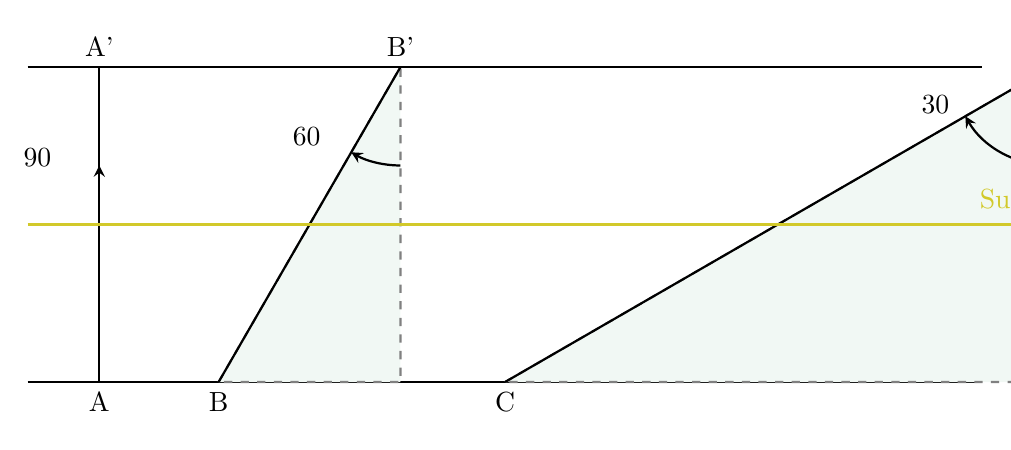
\begin{tikzpicture}[thick]
\def\h{4cm}
\useasboundingbox (0,-.5cm)rectangle(\textwidth,{\h+.5cm});
\draw (0,\h)--+(\textwidth,0);
\draw (0,0)--+(\textwidth,0);
\angLine{90}{.075}{A}
\angLine{60}{.2}{B}
\angLine{30}{.5}{C}
\draw[thick,->,yellow!80!black] (0,.5*\h) -- +(1.05\linewidth,0)node[above]{Sunlight};
\end{tikzpicture}
}

\def\sunTilt{
	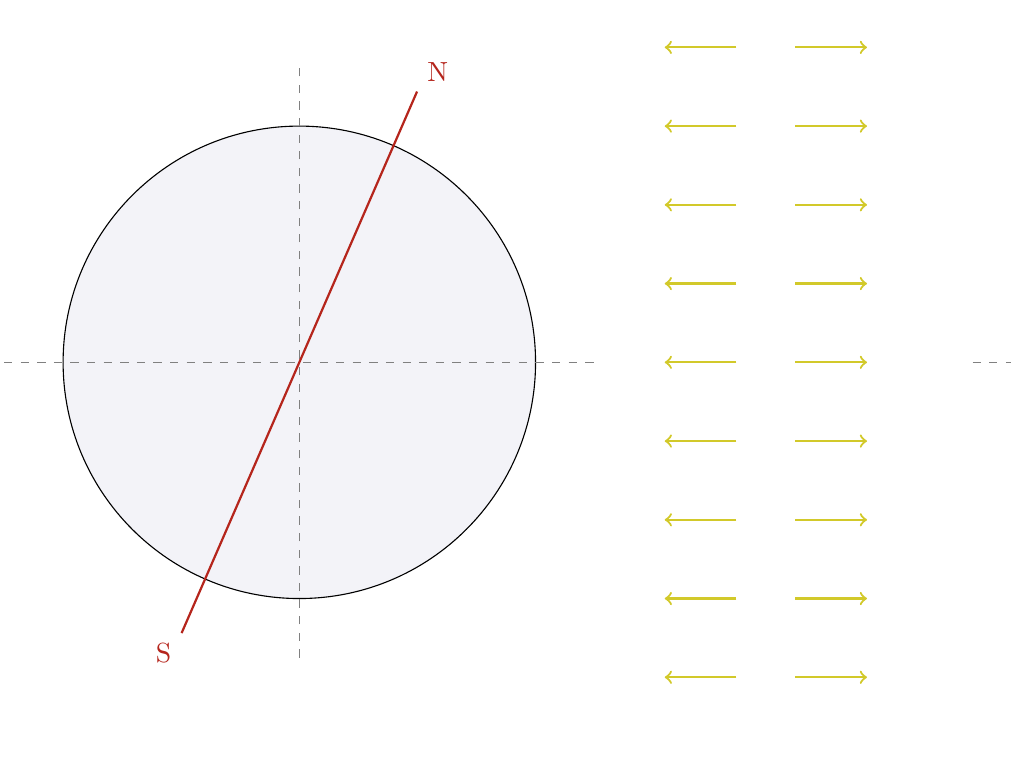
\begin{tikzpicture}
	\def\r{3cm}
	\def\h{2cm}
	\def\planet{
		\draw[fill=MidnightBlue!5] (0,0) circle(\r);
		\draw[dashed, black!50] (180:1.25*\r) -- (0:1.25*\r);
		\draw[dashed, black!50] (-90:1.25*\r) -- (90:1.25*\r);
		\draw[BrickRed, thick] (0,0)++({90-23.5}:1.25*\r)node[above right]{N}--(-{90-23.5}:1.25*\r)node[below left]{S};
	}
	\useasboundingbox (0,-2.5*\h+.25cm)rectangle(\linewidth,2*\h+.25cm);

	\begin{scope}[xshift=1.15*\r,yshift=0]
	\planet
	\end{scope}

	\begin{scope}[xshift=5.25*\r,yshift=0*\r]
	\planet
	\end{scope}

	\begin{scope}[xshift=5.25*\r,yshift=0*\r]
	\foreach \y in {0,...,8}{
		\draw[thick,->,yellow!80!black] (-2.*\r,\y-4) -- + (0.075*\linewidth,0);
		\draw[thick,->,yellow!80!black] (-2.25*\r,\y-4) -- + (-0.075*\linewidth,0);
	};
	\end{scope}
	\end{tikzpicture}
}


\begin{document}
\myTitle{Basic Ocean Navigation}
%------------------------------------------------------------%
%                                                            %
%                          Section                           %
%                                                            %
%------------------------------------------------------------%
\section{Length Along a Circle (Arc Length)}
\begin{minipage}[b]{.5\linewidth}
	Eratosthenes' estimate of the Earth's circumference was based on:
	\begin{enumerate}[(a)]
		\item the length of the shadow cast by the Sun at different locations on the Earth, and
		\item the idea of the circumference of a circle.
	\end{enumerate}
\end{minipage}
\begin{minipage}{0.5\linewidth}
	\pizza
\end{minipage}
So, lets first get to know `the circle' better\ldots
%
\begin{enumerate}[\style (1)]
	\item If the radius of a circle is $R$ how long is its circumference? \answer{$2\pi R$}{2cm}
	\item A `whole' circumference corresponds to 360$\deg$. What arc lengths corresponds to other angles?
\end{enumerate}	\save
\[
\def\ansCell{\cellcolor{gray!10}}
\setlength{\arraycolsep}{.25cm}
\renewcommand{\arraystretch}{2}
\begin{array}{l|*4{>{\cellcolor{white}\quad}c<{\quad}>{\cellcolor{PineGreen!10}\quad}c<{\quad}}}
\text{\textbf{Angle}}  & 360\deg & 180\deg & 90\deg & 45\deg & 10\deg & 1\deg & x\deg \\ \midrule
\text{\textbf{Length of Arc}}& 2 \pi R &  \pi R &\ansCell \answer{$\dfrac{1}{2}\pi R$}{0cm} & \dfrac{1}{4}\pi R &\ansCell  \answer{$\dfrac{1}{6}\pi R$}{0cm} & \dfrac{1}{18}\pi R  &\ansCell \answer{\color{myGreen!10}$\dfrac{x}{180} \pi R$}{0cm} \\
\end{array}
\]
%
%------------------------------------------------------------%
%                                                            %
%                          Section                           %
%                                                            %
%------------------------------------------------------------%
\section{The Size of the Earth}
\begin{enumerate}[\style (1)]\resume
	\item The digram below shows sunlight impinging on the Earth.
	\begin{enumerate}
		\item Indicate the length of the shadows cast by the poles that are positioned at different locations on the Earth.
		\item Use $a$, $b$ and $c$ to indicate the angles between the sunlight and the pole at $A$, $B$ and $C$ respectively.
		\item Indicate and express the angles $\angle COA$ and $\angle COB$ using either $a$, $b$ or $c$.

		\begin{center}
			\begin{tabular}{cccc}
				$\angle COA:$ & \answer{b}{4cm}& $\angle COB:$ & \answer{c}{4cm}
			\end{tabular}
		\end{center}
	\end{enumerate}

	\Erato

	\newpage

	\item Using $\triangle$'s $COB$ and $COA$ and taking the radius of the Earth as $R_E$, write down the distances $CB$ and $CA$.
	\begin{center}
		\begin{tabular}{cccc}
			$CB:$ & \answer{$\dfrac{b}{360}\times 2\pi R_E$}{4cm}& $CA:$ & \answer{$\dfrac{a}{360}\times 2\pi R_E$}{4cm}
		\end{tabular}
	\end{center}
	%
	\item Lets assume $A$ to be Alexandria and $C$ to be Syene.
	\newline Eratosthenes figured out that the angle formed by the shadow at Alexandria (i.e. $a$) is $7^\circ$ and that the distance ($CA$) between the cities is $785$~km.

	Use this information to determine the radius $R_E$ of the Earth.
	\abox{
		\begin{align*}
		CA &= \dfrac{a}{360}\times 2\pi R_E\brk
		\Rightarrow R_E &= \dfrac{360}{a}\times \dfrac{1}{2 \pi} \times CA = \dfrac{360}{7}\times \dfrac{1}{2 \pi} \times 785\text{ km}
		\approx 6204\text{km}
		\end{align*}
	}
	\item Google the value of the Earth's radius. $R_E$ \answer{6371}{3cm}~km. \newline
	(Notice how close Eratosthenes got to the real value over, 2000 years ago!!!)
\end{enumerate}\save
%------------------------------------------------------------%
%                                                            %
%                          Section                           %
%                                                            %
%------------------------------------------------------------%
\section{In the Northern Hemisphere}
\begin{minipage}{0.45\linewidth}
	\begin{enumerate}[\style (1)]\resume
		\item What is special about Polaris (North star)?\brk
		\answer{The Earth's axis of rotation passes through the pole star.}{\linewidth}
		\item Use the diagram to show how we can use\\ Polaris to determine latitude.
	\end{enumerate}\save

	\bigskip
	%------------------------------------------------------------%
	%                                                            %
	%                          Section                           %
	%                                                            %
	%------------------------------------------------------------%
	\section{Time \& Longitude}
	%
	\begin{enumerate}[\style (1)]\resume
		\item Google the longitudes of the following locations and indicate in the table. Also note down the order in which the `new' Sun is observed.
	\end{enumerate}\save
	{
		%\setlength{\tabcolsep}{20pt}
		\renewcommand{\arraystretch}{1.5}
		\begin{tabular}{>{\bfseries}c|*3{C{.275\linewidth}|}}
			& London & San Francisco & Singapore \\
			\toprule
			Longitude & & & \\ \midrule
			Order & & & \\
			\bottomrule
		\end{tabular}
	}
\end{minipage}
\begin{minipage}{0.4\linewidth}
	\globe
\end{minipage}

\bigskip

\begin{enumerate}[\style (1)]\resume
	\begin{minipage}{0.475\linewidth}
		\item Approximately how long will it take\\ `noon' to reach London after Singapore?
		\abox{
			\scriptsize
			\[
			\begin{array}{R{0.55\linewidth}cl}
			Time taken by the Sun to `move' from one meridian to the next (i.e. to move by 1\degree) & = & 4~\text{min} \brk
			Number of meridians between Singapore \& London &= &103.9^{\circ}~\text{E}  - 0.3^{\circ}~\text{E} \\
			&=&103.6^{\circ}\\
			Time necessary for the Sun to move through $103.6^{\circ}$ & = & 4~\frac{\text{min} }{^{\circ}} \times 103.6^{\circ}\\
			&=&414.4~\text{min}\\
			&\approx&6.9~\text{h}
			\end{array}
			\]
		}
		\hfill\scriptsize(answer: 6.9~h)
	\end{minipage}
	%
	\hspace{0.05\linewidth}
	\begin{minipage}{.475\linewidth}
		\item Approximately how long will it take\\ `noon' to reach San Francisco after Singapore?
		\abox{
			\scriptsize
			\[
			\begin{array}{R{0.55\linewidth}cl}
			Time taken by the Sun to `move' from one meridian to the next (i.e. to move by 1\degree) & = & 4~\text{min} \brk
			Number of meridians between Singapore \& San Francisco &= &103.9^{\circ}~\text{E}  + 122.4^{\circ}~\text{W} \\
			&=&226.3^{\circ}\\
			Time necessary for the Sun to move through $103.6^{\circ}$ & = & 4~\frac{\text{min} }{^{\circ}} \times 103.6^{\circ}\\
			&=&905.2~\text{min}\\
			&\approx&15.1~\text{h}
			\end{array}
			\]
		}
		\hfill\scriptsize(answer: 15.1~h)
	\end{minipage}

	\newpage

	\item Mr Bond; Mr \href{https://en.wikipedia.org/wiki/James_Bond}{James Bond}, is in trouble. He just woke up to find himself floating in the middle of the ocean (lucky for him the fancy tuxedo that Q had given him is keeping him warm and afloat). All he remembers is going out to drinks with his `friends' in London, and he is now wondering where he is. He notices that the Sun is not casting a shadow and therefore figures out it should be time for lunch. However, when he looks at his watch, it shows 2 pm! What is 007's present longitude?

	\abox{
		Mr. Bond's watch shows the time in London. If it is 2~pm in London, that means the Sun has moved two-hours worth of meridians towards the west from the location of London. Since, every hour is worth 15\degree, Mr. Bond is at 30\degree E; i.e. in the middle of the Atlantic!
		\vspace{2cm}
	}

\end{enumerate}\save

%------------------------------------------------------------%
%                                                            %
%                          Section                           %
%                                                            %
%------------------------------------------------------------%
\section{Travelling the World}
\subsection{Issues of Time}

\begin{enumerate}[\style (1)]\resume
	\item Do you go `back' or `forward' in time if you travel East or West from your current location\brk
	\begin{inparaenum}
		\item East:\answer{forward}{2cm} \qquad
		\item West:\answer{backwards}{2cm}
	\end{inparaenum}

	\item If the time now is 10:00, what is the time at a location:\brk
	\begin{inparaenum}
		\item 15\degree~East:\answer{11:00}{2cm} \qquad
		\item 15\degree~West:\answer{9:00}{2cm}
	\end{inparaenum}
\end{enumerate}\save

\subsection{Round-the-World Trip!}
\begin{enumerate}[(1)]\resume
	\item \ \\[-2.5em]

	\def\moveU{\underline{M}arvin}\def\stayU{\underline{S}usan}
	\def\move{Marvin}\def\stay{Susan}
	%
	\def\sg{\textbf{Singapore} }
	\def\lon{\textbf{London} }
	\def\san{\textbf{San Francisco} }
	%
	\begin{minipage}{0.5\linewidth}

		\move\ is going on a round-the-world trip and\\ \stayU\ will \underline{s}tay put in Singapore.
		\medskip

		\moveU\ will be \underline{m}oving in quick succession from\newline \sg to \lon to \san and\newline back to \sg.
		\medskip


		The diagram shows (real) flight times and time differences between the cities.
		\textit{Note that the time differences have been (naively) determined using only the differences in longitude.}

		\medskip
		Use the table below to keep track of \move's and \stay's dates \& times during this journey.
	\end{minipage}
	\begin{minipage}{0.5\linewidth}
		\aroundTheWorld
	\end{minipage}
	%
	\bigskip

	{
		\small
		\newcommand{\tD}[2]{{\color{myBrown}{#1}}~on~{\color{myBlue}{#2-Oct}}}
		\rowcolors{4}{white}{MidnightBlue!10}
		\begin{tabular}{>{\bfseries}c|C{3cm}|C{3.2cm}|C{3.cm}||cc}
			\multicolumn{4}{c||}{\textcolor{BrickRed}{\move}}  & \multicolumn{2}{c}{\textcolor{BrickRed}{\stay}} \\
			\toprule
			\rowcolor{PineGreen!15}\bfseries Location &\bfseries  Travel Time\newline to next destination &\bfseries  Time Difference from previous origin& Date-Time\newline on arrival &  &\bfseries  Date-Time in Singapore\\[0.25cm]
			\midrule
			Singapore & - &  - & \vfill\tD{16:00}{11}  \vfill& & \tD{16:00}{11}\brk
			London & \answer{13 h}{0cm} &\answer{-7 h}{0cm} &\vfill\answer{\tD{06:00}{20}}{0cm} \vfill& &\answer{\tD{13:00}{20}}{0cm} \brk
			San Francisco& \answer{11 h}{0cm}& \answer{-8 h}{0cm} &\vfill \answer{\tD{09:00}{20}}{0cm} \vfill &&\answer{\tD{0:00}{21}}{0cm}\brk
			Singapore& \answer{18 h}{0cm} & \answer{-9 h}{0cm} &\vfill \answer{\tD{18:00}{20}}{0cm} \vfill & &\answer{\tD{18:00}{21}}{0cm}\brk
			\bottomrule
		\end{tabular}
	}

	\smallskip
	Do you now see why you should be conscious of how you cross the international date line.

\end{enumerate}\save


%------------------------------------------------------------%
%                                                            %
%                          Section                           %
%                                                            %
%------------------------------------------------------------%
\section{23$\dfrac{1}{2}$\degree~ Tilt}
\sunTilt
\begin{enumerate}[\style (1)] \resume

	\item The two diagrams show how sunlight hits the Earth in the months of June and December.

	Identify which diagram corresponds to which month.

	\item Indicate the locations of the Sun and the North Star (Polaris).

	\item Indicate the positions of the Equator, the Tropic of Capricorn and the Tropic of Cancer.

	\item Indicate the angles at which sunlight falls on the above three locations.

\end{enumerate}

\end{document}
